% ********** Rozdział 3 **********
\chapter{Realizowanie \&\& warstwa projektu}
\section{Diagram Gantta}
\begin{figure}[!ht]
	\centering
		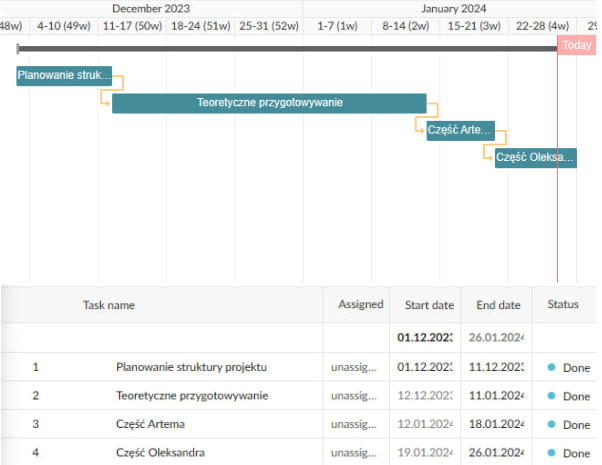
\includegraphics[width=16cm]{gantt.jpg}
  \caption{\footnotesize Realizowanie projektu}
	\label{fig:plotend}
\end{figure}
Z diagramu widać, że najpierw przez 10 dni planowaliśmy projekt i omawialiśmy, co będziemy realizowali jako pierwsza wersja aplikacji. Zaten przygotowywanie zajęło dużo czasu, po czym zaczęliśmy pisać kod projektu, najpierw Pan Artem i pozostałe realizowałem sam.
\newpage
\section{Prezentacja warstwy projektu}
\begin{figure}[!ht]
	\centering
		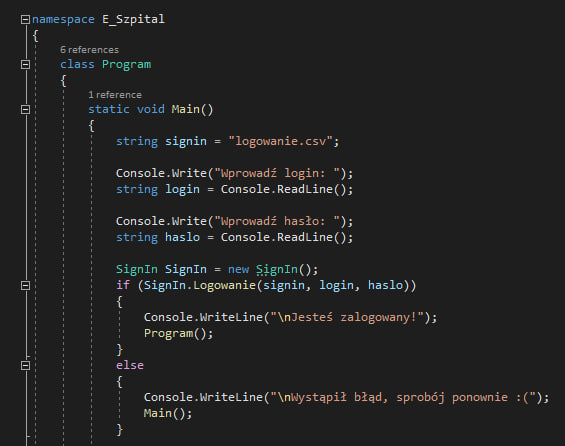
\includegraphics[width=16cm]{E-Szpital/oop1.jpg}
	\caption{\footnotesize Logowanie do aplikacji}
	\label{fig:plotend}
\end{figure}\newline
Na starcie projektu od razu wita nas logowanie, w tym celu pobieramy Login i Hasło za pomocą\\ ReadLine, a za pomocą metody Logowanie sprawdzamy czy hasło i login wpisane przez użytkownika znajdują się w bazie danych.\newpage Metoda Logowanie wygląda następująco: znajduje się w klasie SignIn, i pobiera ścieżkę do bazy loginów i haseł. Metoda tworzy tablicę z danych znajdujących się w bazie i porównuje dostępne dane z danymi wprowadzonymi przez użytkownika za pomocą foreach. Jeśli dane się zgadzają, metoda zwraca wartość true. Jeśli nie, false
\newline
\begin{figure}[!ht]
	\centering
		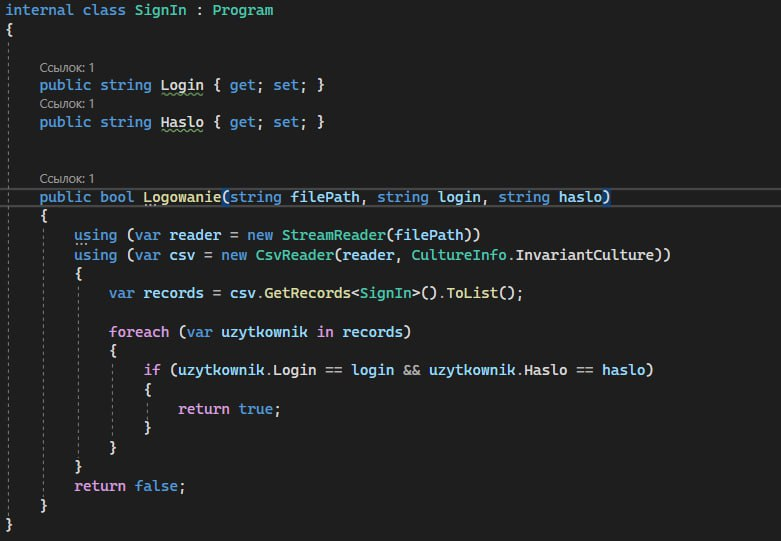
\includegraphics[width=16cm]{E-Szpital/signin.jpg}
	\caption{\footnotesize Metoda logowania}
	\label{fig:plotend}
\end{figure}\newpage
W tym miejscu znajdują się niezbędne lokalne zmienne, stworzone do wyjaśnienia aplikacji, z których plików csv pobierać lub zapisywać informacje, również lokalne zmienne do korzystania z metod, które są stworzone w klasach. \newline
\begin{figure}[!ht]
	\centering
		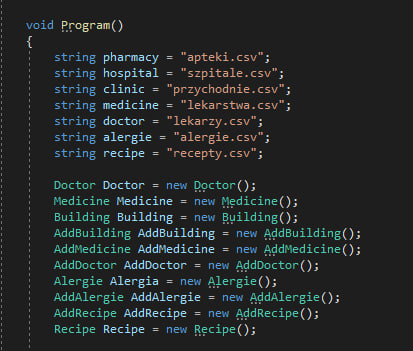
\includegraphics[width=16cm]{E-Szpital/oop2.jpg}
	\caption{\footnotesize Programowe niezbędności}
	\label{fig:plotend}
\end{figure}\newpage
Główne menu ma 8 opcje, 6 do korzystania jako użytkownik: wyświetlenie informacji o aptekach, szpitalach, przychodniach, lekach, lekarzach i alergiach. Oraz "7. Dodaj" służy do up-date`u aplikacji z możliwością dodawać nowe dane do bazy. Zwykły ReadLine do wyboru opcji z wpisanej wartości. \newline
\begin{figure}[!ht]
	\centering
		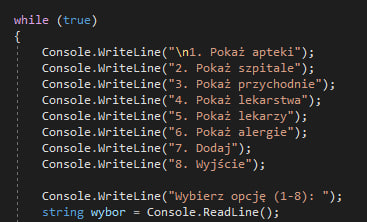
\includegraphics[width=16cm]{E-Szpital/oop3.jpg}
	\caption{\footnotesize Główne menu}
	\label{fig:plotend}
\end{figure}\newpage
Tak wygląda rozwinięcie opcji 1, czyli "Pokaż apteki", stworzone opcje wyszukiwania z nazwy, dzielnicy oraz wyświetlenie wszystkich aptek z bazy danych. W tym bloku głównie działa wszystko odwołując do metod, stworzonych w klasie "Building", które pokazane są dalej. \newline
\begin{figure}[!ht]
	\centering
		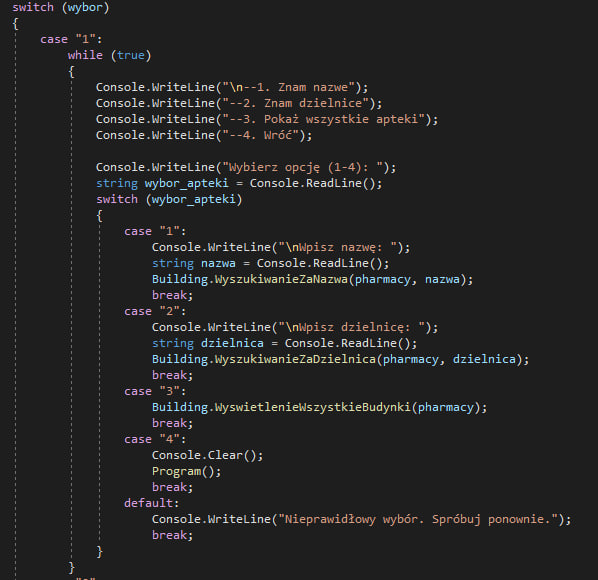
\includegraphics[width=16cm]{E-Szpital/oop4.jpg}
	\caption{\footnotesize Pokaż apteki}
	\label{fig:plotend}
\end{figure}\newpage

Biblioteki CSVhelper, CSVhelper.Configuration umożliwiają stworzenie metody do uzyskania dostępu do danych z pliku csv. Var`y reader i csv służą do wyszukiwania potrzebnego pliku, łącznie z odwołaniem do var pharmacy, pokazanego już wcześniej. Var records pobiera wpisywane dane do sprawdzania, czy są w pliku.\newline
\begin{figure}[!ht]
	\centering
		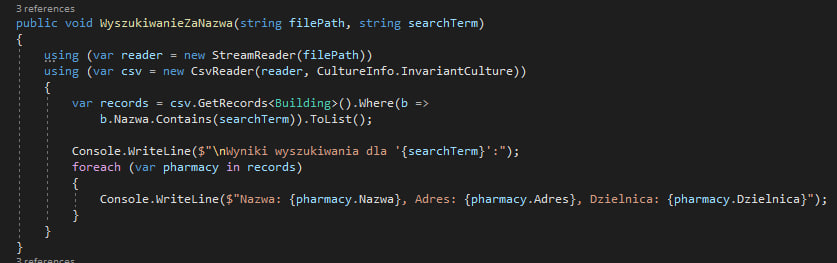
\includegraphics[width=16cm]{E-Szpital/oop5.jpg}
	\caption{\footnotesize Metoda wyszukiwania za nazwą}
	\label{fig:plotend}
\end{figure}\newline
Wyświetlenie wszystkich budynków różnie się w var records, bez sprawdzania istnienia wpisanych danych w pliku, pokazując wszystko po kolei.\newline
W podobny sposób byli napisane inne wyszukiwania z różnicami dt. danych, przykładowo leki do wyszukiwania mają atrybuty "nazwa","producent"\ i "kategoria"; lekarz - "imie", "nazwisko"\\\ i "specjalność" i t.d. Żeby zaoszędzić troche czasu pominiemy pokazywanie wykorzystanie z takich samych formuł tworzenia metod.\newline
\begin{figure}[!ht]
	\centering
		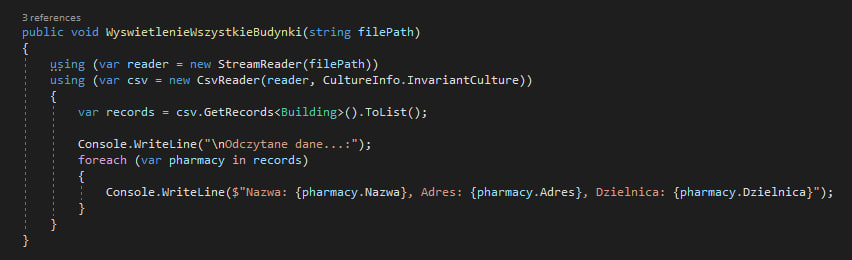
\includegraphics[width=16cm]{E-Szpital/oop6.jpg}
	\caption{\footnotesize Metoda wyświetlenia wszystkich danych}
	\label{fig:plotend}
\end{figure}\newpage
\begin{figure}[!ht]
	\centering
		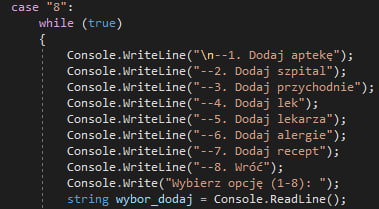
\includegraphics[width=14cm]{E-Szpital/oop7.jpg}
	\caption{\footnotesize Menu dodawania nowych danych}
	\label{fig:plotend}
\end{figure}\newline
Tak samo za pomocy bibliotek CSVhelper, CSVhelper.Configuration stworzone są metody do dodania nowej informacji do plików, z których korzysta aplikacja, do których tutaj wpisane są odwołania.\newline
\begin{figure}[!ht]
	\centering
		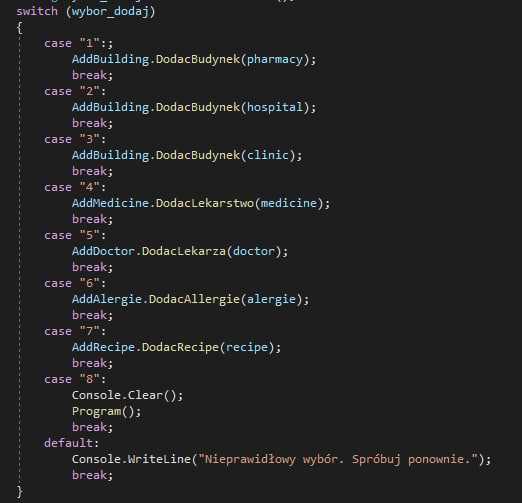
\includegraphics[width=14cm]{E-Szpital/oop8.jpg}
	\caption{\footnotesize Odwołania do metod}
	\label{fig:plotend}
\end{figure}\newpage
\begin{figure}[!ht]
	\centering
		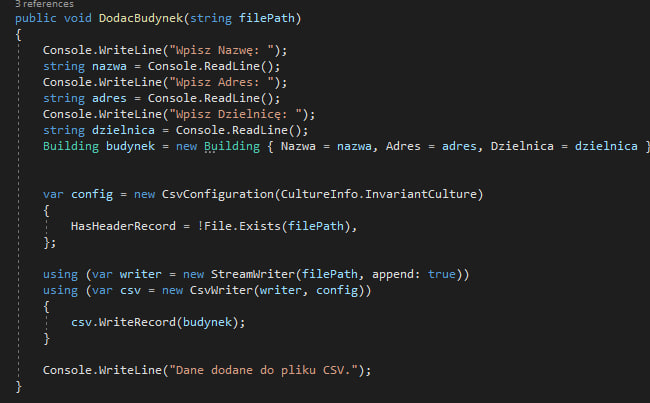
\includegraphics[width=14cm]{E-Szpital/oop9.jpg}
	\caption{\footnotesize Metoda dodawania nowych danych}
	\label{fig:plotend}
\end{figure}\newline
Podobnie do tego screenu, używając readline do pobierania wpisywanych danych od użytkowniku, stwarza się obiekt klasy "Building" i za pomocy csvhelper rzucamy ten obiekt do bazy danych.\newpage

\subsubsection{Żródła plików}
\begin{figure}[!ht]
	\centering
		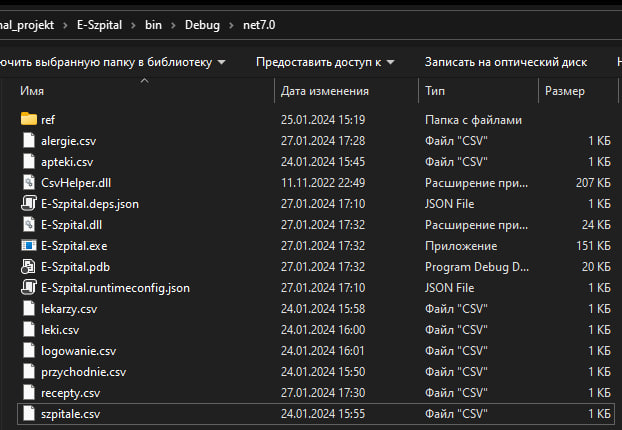
\includegraphics[width=16cm]{E-Szpital/net7.jpg}
	\caption{\footnotesize Pliki używane aplikacją}
	\label{fig:plotend}
\end{figure}\newline
\begin{figure}[!ht]
	\centering
		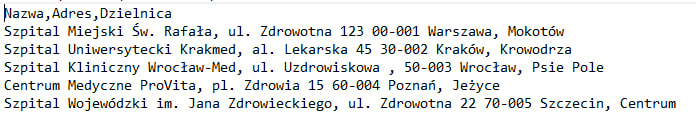
\includegraphics[width=16cm]{E-Szpital/szpital.jpg}
	\caption{\footnotesize Tekst w pliku szpital.csv}
	\label{fig:plotend}
\end{figure}\newline
I tutaj widoczne jest, jak wygląda tekst, który rozumie aplikacja i biblioteki powiązanie z csv. W podobny sposób zrobione są pozostałe.
\newpage\subsection{Podalsze plany}
Dalsze rozwinięcie projektu łączy w sobie pracę nad interfejsem, funkcjonalnością, dodawanie nowych metod i potencjalnie testowanie gotowej wercji (do tego jeszcze długo).
% ********** Koniec rozdziału **********
